\documentclass{beamer}
\usetheme{Berlin}
\usepackage{multimedia}
\usepackage[magyar, english]{babel}
\usepackage{t1enc}

\title{A lítiumion-akkumulátorok működése és felhasználása}
\author{Vitkolczi Dániel, Nagy Balázs}
\date{}

\begin{document}

\section*{Bevezetés}
\begin{frame}
\titlepage
\end{frame}

\begin{frame}
\frametitle{Előretekintés}
\tableofcontents
\end{frame}

\section{Rövid összefoglalás az előadásról}
\begin{frame}
\frametitle{Az előadás témája}
\textbf{Az előadásban megemlítésre kerülő témák:}\\~\\
\begin{enumerate}
	\item<1-> Elemek általános működésének elve
	\item<2-> A lítium atom hasznos tulajdonságai
	\item<3-> Lítiumionos elemek alapelve és működése
	\item<4-> Felhasználásuk a mindennapokban
	\item<5-> A közeljövőre vonatkozó lehetséges applikációk
\end{enumerate}
\end{frame}

\section{Miért pont lítium?}
\begin{frame}
\frametitle{Gyorstalpaló}
\begin{center}
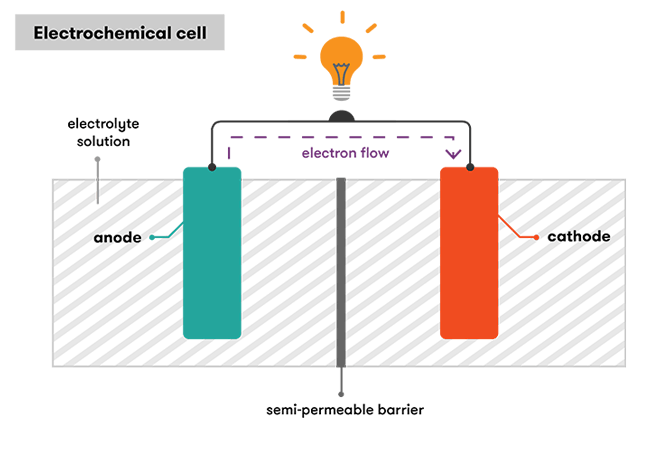
\includegraphics[scale=0.26]{battery}
\end{center}

\begin{block}{Anód és Katód}
	Az katód egy negatív töltésű elektróda, amely az elektronokat szolgáltatja, az anód pedig pozitív töltésű, így az befogadja az elektronokat. 
\end{block}
\end{frame}

\begin{frame}
\begin{columns}
	\begin{column}{0.5\textwidth}
		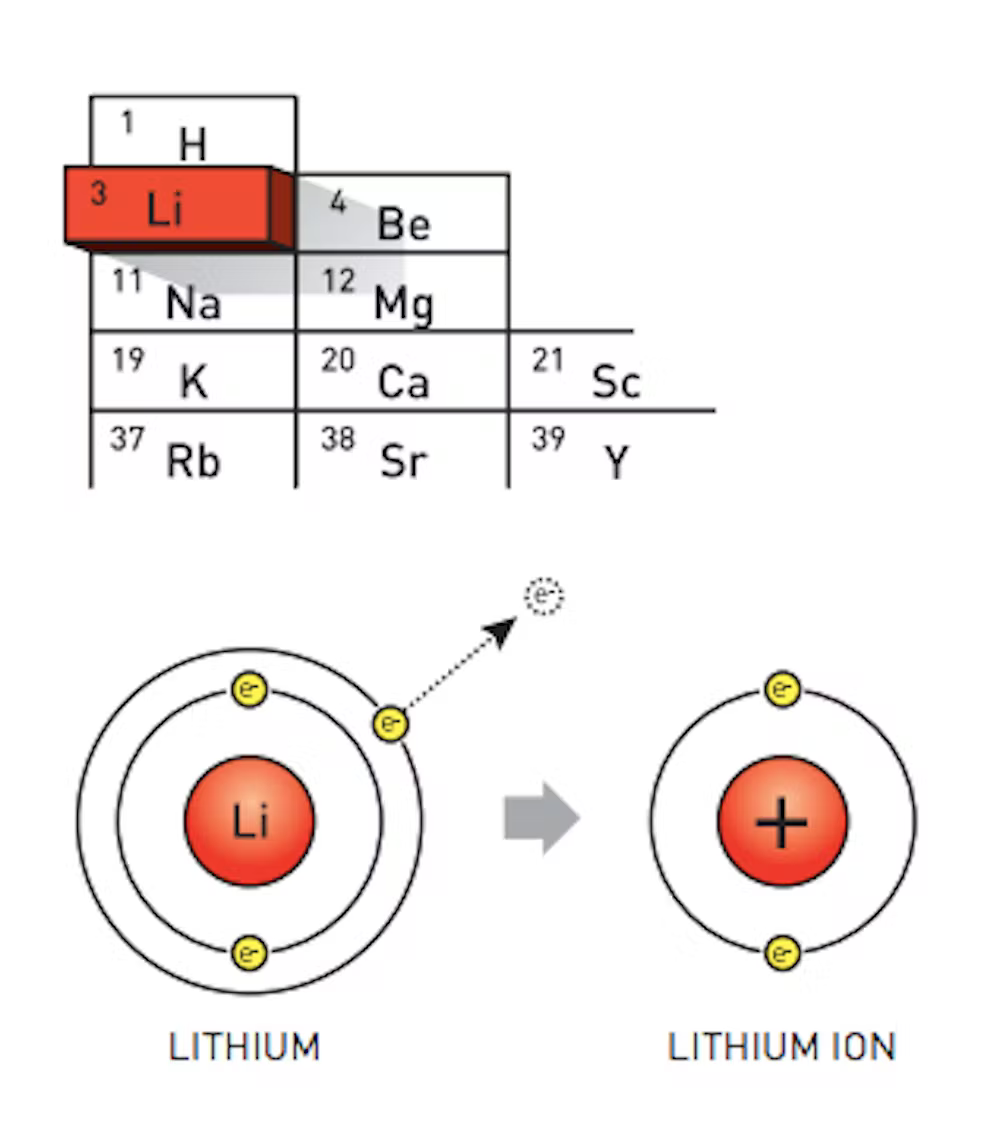
\includegraphics[scale=0.2]{lithiumion}
	\end{column}
	\begin{column}{0.4\textwidth}
		\begin{block}{Ion}
			Olyan atom vagy molekula, mely elektromos töltéssel rendelkezik.
		\end{block}
	\end{column}
\end{columns}
\end{frame}

\begin{frame}
\frametitle{A lítium tulajdonságai}
\begin{block}{Általános jellemzők}
\begin{itemize}
\item \textbf{Neve:} Lítium (ógörög: lithosz, ómagyar: lavany)
\item \textbf{Vegyjel:} Li
\item Fekete színű, ásványi olajban kell tárolni
\item 3. elem a peridósusos rendszerben, legelső és legkisebb sűrűségű fém, első szilárd elem (standard körülmények között)
\item Instabil atommag, az egyetlen könnyűfém, ami maghasadásra képes
\item 2 stabil izotóp: 6-os és a 7-es izotóp, ebből a 7-es a gyakoribb 92,5%-os relatív gyakorisággal
\end{itemize}
\end{block}
\end{frame}

\begin{frame}
\begin{block}{Miért jó akkumulátorokba}
\begin{itemize}
\item A legerősebb redukálószer, tehát legjobb anód
\item Nagyon könnyű (16-szor kisebb a sűrűsége a nikkelnél)
\end{itemize}
\end{block}

\begin{block}{Mi a probléma}
\begin{itemize}
\item Relatív kevés van belőle: Az első 32 elemből csak a 26-ik leggyakoribb. Nagy része az óceánokban van feloldódva. A sósivatagok a legjobb lelőhelyek közé tartoznak.
\end{itemize}
\end{block}
\end{frame}

\begin{frame}
\frametitle{
Jobb-e mint a hagyományos}
\begin{block}{Mellette}
\begin{itemize}
\item Környezet barátabb (mindent összevetve, átlagosan 30\%-al jobb egy elektronikus autónak a klíma mérlege)
\end{itemize}
\end{block}

\begin{block}{Ellene}
\begin{itemize}
\item Rendkívül környezetszennyező magának a lítiumnak a bányászata
\item Az akkumulátorok nem újrahasznosíthatóak
\item Nem oljda meg az energia válságot
\end{itemize}
\end{block}
\end{frame}

\begin{frame}
\frametitle{Az elemek általános működése}
\begin{center}
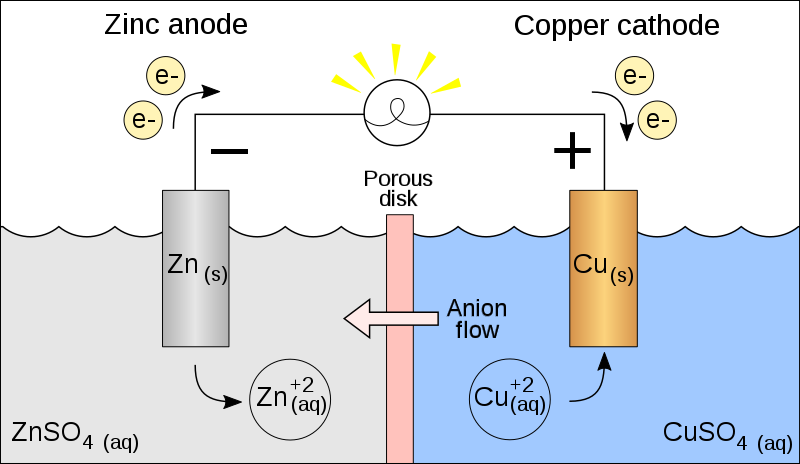
\includegraphics[scale=0.3]{galvanicbattery}
\end{center}
\end{frame}

\begin{frame}
\frametitle{Elemekben való implementáció (Élettartam)}
\begin{center}
	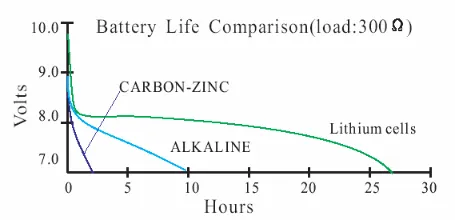
\includegraphics[scale=0.5]{batterylife}
\end{center}
\begin{center}
	\textbf{\textit{A lítiumionos-akkumulátorok élettartamának összehasonlítása más típusú akkumulátorokhoz képest}}
\end{center}
\end{frame}

\begin{frame}
\frametitle{Elemekben való implementáció (Hatákonyság)}
\begin{center}
	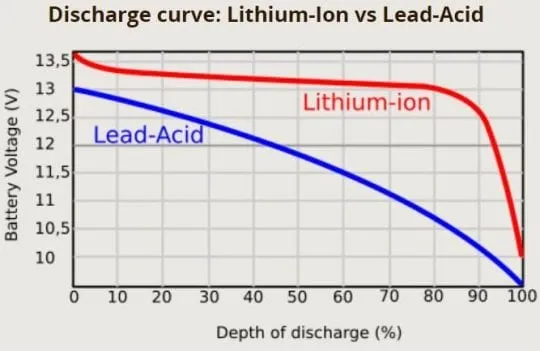
\includegraphics[scale=0.4]{discharge}
\end{center}
\begin{center}
	\textbf{\textit{Az akkumulátor által eltárolt töltés fogyásának a mértéke}}
\end{center}
\end{frame}

\section{A lítium ionos elemek működése}
\begin{frame}
\frametitle{Implementáció, működési alapelve}
\begin{center}
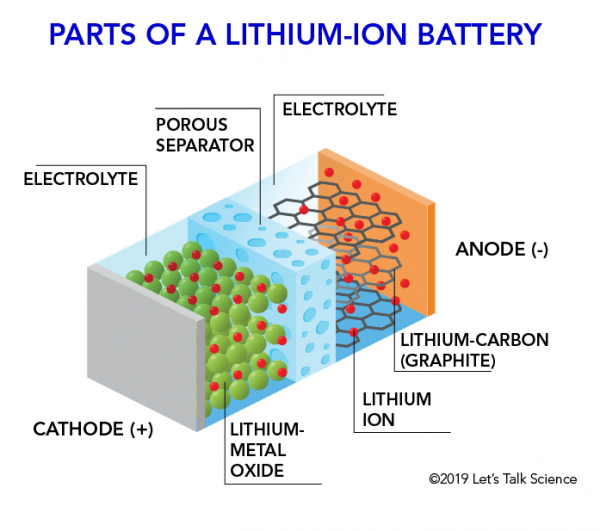
\includegraphics[scale=0.5]{batterycutaway}
\end{center}
\end{frame}

\begin{frame}
\frametitle{Elemek merülése}
\begin{center}
	VIDEO
\end{center}
\end{frame}

\begin{frame}
\frametitle{Elemek töltése}
\begin{center}
	VIDEO
\end{center}
\end{frame}

\section{Felhasználásuk és előrelátható alkalmazásuk}
\begin{frame}
\frametitle{A lítiumion-akkumulátorok alkalmazása}
\begin{columns}
\begin{column}{0.5\textwidth}
\begin{enumerate}
\item<1-> Elektromos járművek
\item<2-> Hordozható eszközök
\item<3-> Elektromos szerszámok
\item<4-> És még sok más helyen
\end{enumerate}
\end{column}
\begin{column}{0.5\textwidth}
\includegraphics<1>[scale=0.3]{car}
\includegraphics<2>[scale=0.4]{phone}
\includegraphics<3>[scale=0.5]{drill}
\includegraphics<4>[scale=0.12]{rover}
\end{column}
\end{columns}
\end{frame}

\begin{frame}
\frametitle{Kitekintés a jövőbe}
\begin{center}
\includegraphics<1>[scale=0.267]{chart}
\includegraphics<2>[scale=0.26]{plane}
\end{center}
\end{frame}

\begin{frame}
\begin{center}
\textbf{\Huge{Köszönjük a figyelmet!}}
\end{center}
\end{frame}

\end{document}